% Options for packages loaded elsewhere
\PassOptionsToPackage{unicode}{hyperref}
\PassOptionsToPackage{hyphens}{url}
\PassOptionsToPackage{dvipsnames,svgnames,x11names}{xcolor}
%
\documentclass[
  letterpaper,
  DIV=11,
  numbers=noendperiod]{scrartcl}

\usepackage{amsmath,amssymb}
\usepackage{iftex}
\ifPDFTeX
  \usepackage[T1]{fontenc}
  \usepackage[utf8]{inputenc}
  \usepackage{textcomp} % provide euro and other symbols
\else % if luatex or xetex
  \usepackage{unicode-math}
  \defaultfontfeatures{Scale=MatchLowercase}
  \defaultfontfeatures[\rmfamily]{Ligatures=TeX,Scale=1}
\fi
\usepackage{lmodern}
\ifPDFTeX\else  
    % xetex/luatex font selection
\fi
% Use upquote if available, for straight quotes in verbatim environments
\IfFileExists{upquote.sty}{\usepackage{upquote}}{}
\IfFileExists{microtype.sty}{% use microtype if available
  \usepackage[]{microtype}
  \UseMicrotypeSet[protrusion]{basicmath} % disable protrusion for tt fonts
}{}
\makeatletter
\@ifundefined{KOMAClassName}{% if non-KOMA class
  \IfFileExists{parskip.sty}{%
    \usepackage{parskip}
  }{% else
    \setlength{\parindent}{0pt}
    \setlength{\parskip}{6pt plus 2pt minus 1pt}}
}{% if KOMA class
  \KOMAoptions{parskip=half}}
\makeatother
\usepackage{xcolor}
\setlength{\emergencystretch}{3em} % prevent overfull lines
\setcounter{secnumdepth}{5}
% Make \paragraph and \subparagraph free-standing
\ifx\paragraph\undefined\else
  \let\oldparagraph\paragraph
  \renewcommand{\paragraph}[1]{\oldparagraph{#1}\mbox{}}
\fi
\ifx\subparagraph\undefined\else
  \let\oldsubparagraph\subparagraph
  \renewcommand{\subparagraph}[1]{\oldsubparagraph{#1}\mbox{}}
\fi

\usepackage{color}
\usepackage{fancyvrb}
\newcommand{\VerbBar}{|}
\newcommand{\VERB}{\Verb[commandchars=\\\{\}]}
\DefineVerbatimEnvironment{Highlighting}{Verbatim}{commandchars=\\\{\}}
% Add ',fontsize=\small' for more characters per line
\usepackage{framed}
\definecolor{shadecolor}{RGB}{241,243,245}
\newenvironment{Shaded}{\begin{snugshade}}{\end{snugshade}}
\newcommand{\AlertTok}[1]{\textcolor[rgb]{0.68,0.00,0.00}{#1}}
\newcommand{\AnnotationTok}[1]{\textcolor[rgb]{0.37,0.37,0.37}{#1}}
\newcommand{\AttributeTok}[1]{\textcolor[rgb]{0.40,0.45,0.13}{#1}}
\newcommand{\BaseNTok}[1]{\textcolor[rgb]{0.68,0.00,0.00}{#1}}
\newcommand{\BuiltInTok}[1]{\textcolor[rgb]{0.00,0.23,0.31}{#1}}
\newcommand{\CharTok}[1]{\textcolor[rgb]{0.13,0.47,0.30}{#1}}
\newcommand{\CommentTok}[1]{\textcolor[rgb]{0.37,0.37,0.37}{#1}}
\newcommand{\CommentVarTok}[1]{\textcolor[rgb]{0.37,0.37,0.37}{\textit{#1}}}
\newcommand{\ConstantTok}[1]{\textcolor[rgb]{0.56,0.35,0.01}{#1}}
\newcommand{\ControlFlowTok}[1]{\textcolor[rgb]{0.00,0.23,0.31}{#1}}
\newcommand{\DataTypeTok}[1]{\textcolor[rgb]{0.68,0.00,0.00}{#1}}
\newcommand{\DecValTok}[1]{\textcolor[rgb]{0.68,0.00,0.00}{#1}}
\newcommand{\DocumentationTok}[1]{\textcolor[rgb]{0.37,0.37,0.37}{\textit{#1}}}
\newcommand{\ErrorTok}[1]{\textcolor[rgb]{0.68,0.00,0.00}{#1}}
\newcommand{\ExtensionTok}[1]{\textcolor[rgb]{0.00,0.23,0.31}{#1}}
\newcommand{\FloatTok}[1]{\textcolor[rgb]{0.68,0.00,0.00}{#1}}
\newcommand{\FunctionTok}[1]{\textcolor[rgb]{0.28,0.35,0.67}{#1}}
\newcommand{\ImportTok}[1]{\textcolor[rgb]{0.00,0.46,0.62}{#1}}
\newcommand{\InformationTok}[1]{\textcolor[rgb]{0.37,0.37,0.37}{#1}}
\newcommand{\KeywordTok}[1]{\textcolor[rgb]{0.00,0.23,0.31}{#1}}
\newcommand{\NormalTok}[1]{\textcolor[rgb]{0.00,0.23,0.31}{#1}}
\newcommand{\OperatorTok}[1]{\textcolor[rgb]{0.37,0.37,0.37}{#1}}
\newcommand{\OtherTok}[1]{\textcolor[rgb]{0.00,0.23,0.31}{#1}}
\newcommand{\PreprocessorTok}[1]{\textcolor[rgb]{0.68,0.00,0.00}{#1}}
\newcommand{\RegionMarkerTok}[1]{\textcolor[rgb]{0.00,0.23,0.31}{#1}}
\newcommand{\SpecialCharTok}[1]{\textcolor[rgb]{0.37,0.37,0.37}{#1}}
\newcommand{\SpecialStringTok}[1]{\textcolor[rgb]{0.13,0.47,0.30}{#1}}
\newcommand{\StringTok}[1]{\textcolor[rgb]{0.13,0.47,0.30}{#1}}
\newcommand{\VariableTok}[1]{\textcolor[rgb]{0.07,0.07,0.07}{#1}}
\newcommand{\VerbatimStringTok}[1]{\textcolor[rgb]{0.13,0.47,0.30}{#1}}
\newcommand{\WarningTok}[1]{\textcolor[rgb]{0.37,0.37,0.37}{\textit{#1}}}

\providecommand{\tightlist}{%
  \setlength{\itemsep}{0pt}\setlength{\parskip}{0pt}}\usepackage{longtable,booktabs,array}
\usepackage{calc} % for calculating minipage widths
% Correct order of tables after \paragraph or \subparagraph
\usepackage{etoolbox}
\makeatletter
\patchcmd\longtable{\par}{\if@noskipsec\mbox{}\fi\par}{}{}
\makeatother
% Allow footnotes in longtable head/foot
\IfFileExists{footnotehyper.sty}{\usepackage{footnotehyper}}{\usepackage{footnote}}
\makesavenoteenv{longtable}
\usepackage{graphicx}
\makeatletter
\def\maxwidth{\ifdim\Gin@nat@width>\linewidth\linewidth\else\Gin@nat@width\fi}
\def\maxheight{\ifdim\Gin@nat@height>\textheight\textheight\else\Gin@nat@height\fi}
\makeatother
% Scale images if necessary, so that they will not overflow the page
% margins by default, and it is still possible to overwrite the defaults
% using explicit options in \includegraphics[width, height, ...]{}
\setkeys{Gin}{width=\maxwidth,height=\maxheight,keepaspectratio}
% Set default figure placement to htbp
\makeatletter
\def\fps@figure{htbp}
\makeatother

\KOMAoption{captions}{tableheading}
\makeatletter
\@ifpackageloaded{caption}{}{\usepackage{caption}}
\AtBeginDocument{%
\ifdefined\contentsname
  \renewcommand*\contentsname{Table of contents}
\else
  \newcommand\contentsname{Table of contents}
\fi
\ifdefined\listfigurename
  \renewcommand*\listfigurename{List of Figures}
\else
  \newcommand\listfigurename{List of Figures}
\fi
\ifdefined\listtablename
  \renewcommand*\listtablename{List of Tables}
\else
  \newcommand\listtablename{List of Tables}
\fi
\ifdefined\figurename
  \renewcommand*\figurename{Figure}
\else
  \newcommand\figurename{Figure}
\fi
\ifdefined\tablename
  \renewcommand*\tablename{Table}
\else
  \newcommand\tablename{Table}
\fi
}
\@ifpackageloaded{float}{}{\usepackage{float}}
\floatstyle{ruled}
\@ifundefined{c@chapter}{\newfloat{codelisting}{h}{lop}}{\newfloat{codelisting}{h}{lop}[chapter]}
\floatname{codelisting}{Listing}
\newcommand*\listoflistings{\listof{codelisting}{List of Listings}}
\makeatother
\makeatletter
\makeatother
\makeatletter
\@ifpackageloaded{caption}{}{\usepackage{caption}}
\@ifpackageloaded{subcaption}{}{\usepackage{subcaption}}
\makeatother
\ifLuaTeX
  \usepackage{selnolig}  % disable illegal ligatures
\fi
\usepackage{bookmark}

\IfFileExists{xurl.sty}{\usepackage{xurl}}{} % add URL line breaks if available
\urlstyle{same} % disable monospaced font for URLs
\hypersetup{
  pdftitle={Parallelizing DIPY model fits with Ray},
  colorlinks=true,
  linkcolor={blue},
  filecolor={Maroon},
  citecolor={Blue},
  urlcolor={Blue},
  pdfcreator={LaTeX via pandoc}}

\title{Parallelizing DIPY model fits with Ray}
\author{Ariel Rokem \and Asa Gilmore}
\date{}

\begin{document}
\maketitle

\section{🚧 Under construction 🚧}\label{under-construction}

\section{Abstract}\label{abstract}

\section{Introduction}\label{introduction}

Ray is a great system for parallelization
(https://arxiv.org/abs/1712.05889).

\section{Methods}\label{methods}

We ran both a constrained spherical deconvolution model and a free water
diffusion tensor model through DIPY on a subject from the human
connectome project (add more about hcp). We created a docker image to
encapsulate the test and allow for easy reproducibility of the tests.
The testing program computes each model 5 times for each set of unique
parameters. We then iterate across chunk sizes exponentially, from 1-15,
where the number of chunks is 2\^{}x (explain better). We ran the tests
with the following arguments on docker instances with CPU counts, 8, 16,
32, 48, and 72:

\begin{verbatim}
--models csdm fwdtim --min_chunks 1 --max_chunks 15 --num_runs 5
\end{verbatim}

\section{Results}\label{results}

Parallelization with \texttt{ray} provided considerable speedups over
serial excicution for both constrained sperical deconvolution models and
free water models. We saw a much greater speedup for the free water
model, which is possibly explained by the fact that it is much more
computationally expensive per voxel. This would mean that the overhead
from parallelizing the model would have a smaller effect on the runtime.
Interestlingly 48 and 72 core instances performed slightly worse than
the 32 core instance on the csdm model, which may indicate that there is
some increased overhead for each core, separate from the overhead for
each task sent to ray.

\begin{longtable}[]{@{}
  >{\raggedright\arraybackslash}p{(\columnwidth - 2\tabcolsep) * \real{0.5000}}
  >{\raggedright\arraybackslash}p{(\columnwidth - 2\tabcolsep) * \real{0.5000}}@{}}
\toprule\noalign{}
\endhead
\bottomrule\noalign{}
\endlastfoot
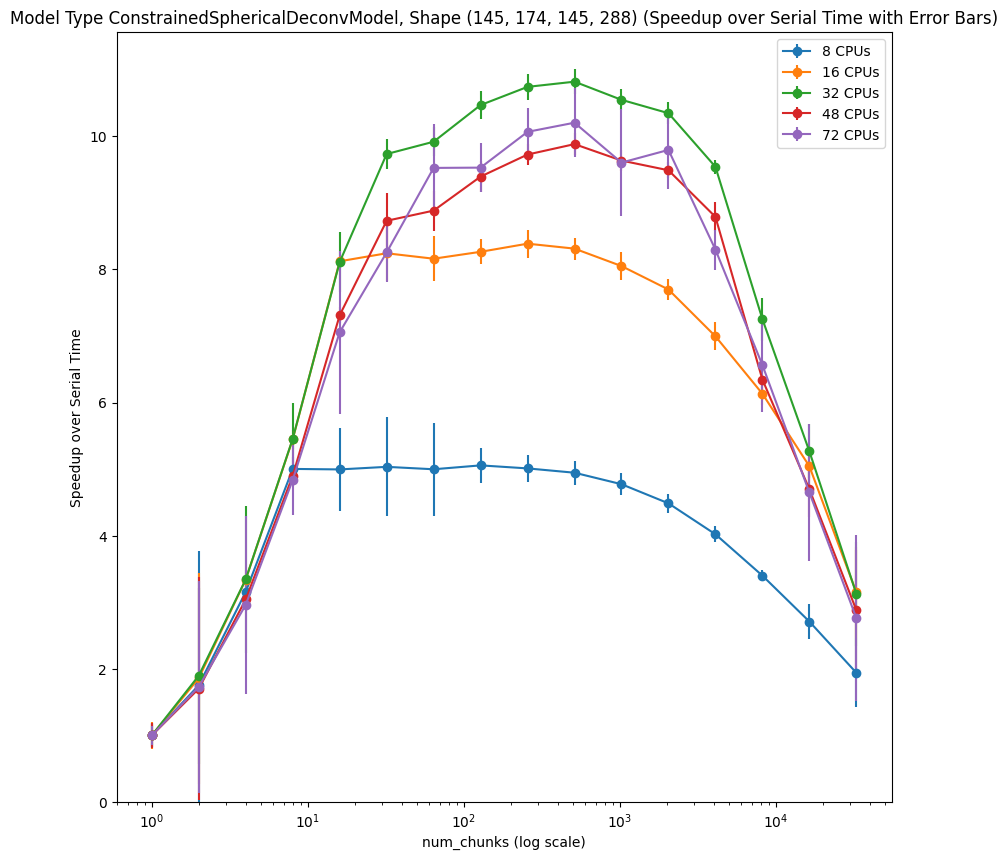
\includegraphics[width=0.8\textwidth,height=0.8\textheight]{figures/csdm_speedup.png}
&
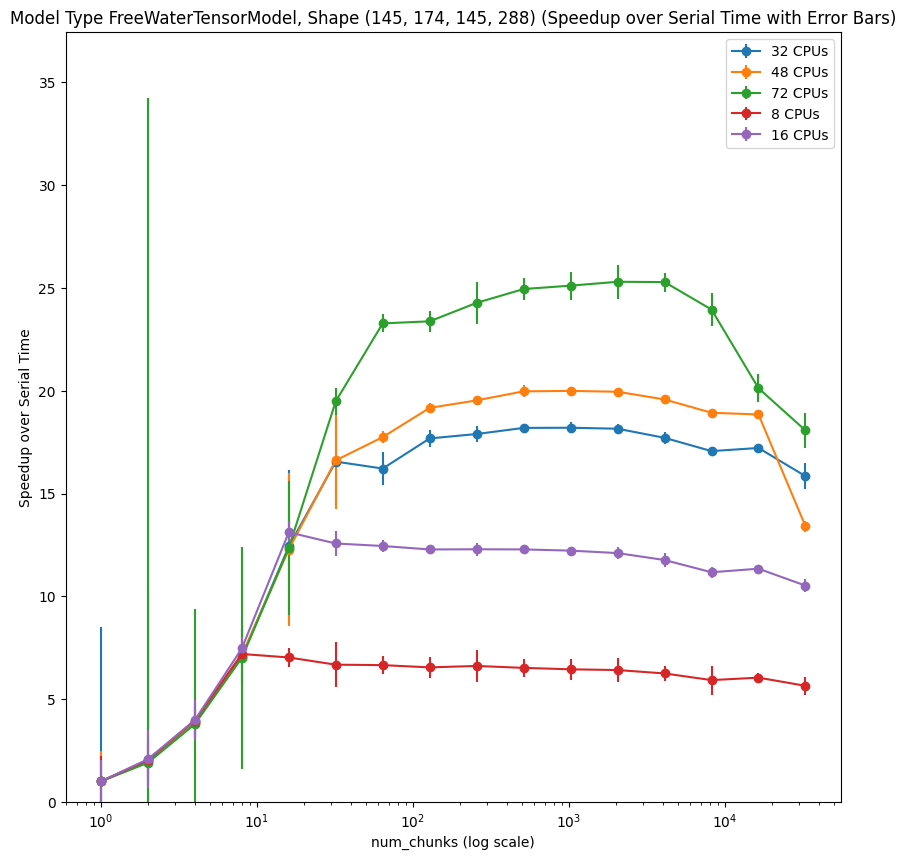
\includegraphics[width=0.8\textwidth,height=0.8\textheight]{figures/fwdtim_speedup.png} \\
\end{longtable}

Efficiency decreases as a function of number of CPUs, but is still
rather high in many configurations. Efficiency is also considerably
higher for the free water tensor model, which is consistent with out
expectations given that it is more computationally expensive per voxel
and therefor ray overhead would have less effect. The high efficency of
8 core machines suggest that the most cost effective configuration for
processing may be relativly cheap low core machines.

\begin{longtable}[]{@{}
  >{\raggedright\arraybackslash}p{(\columnwidth - 2\tabcolsep) * \real{0.5000}}
  >{\raggedright\arraybackslash}p{(\columnwidth - 2\tabcolsep) * \real{0.5000}}@{}}
\toprule\noalign{}
\endhead
\bottomrule\noalign{}
\endlastfoot
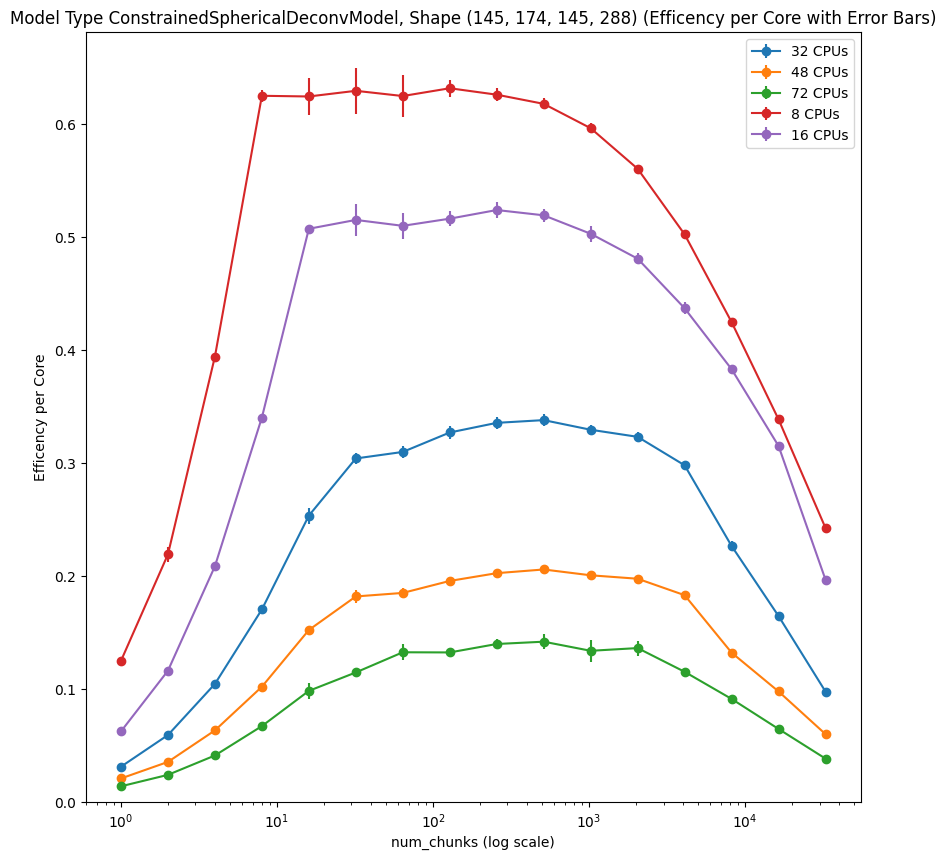
\includegraphics[width=0.8\textwidth,height=0.8\textheight]{figures/csdm_efficency.png}
&
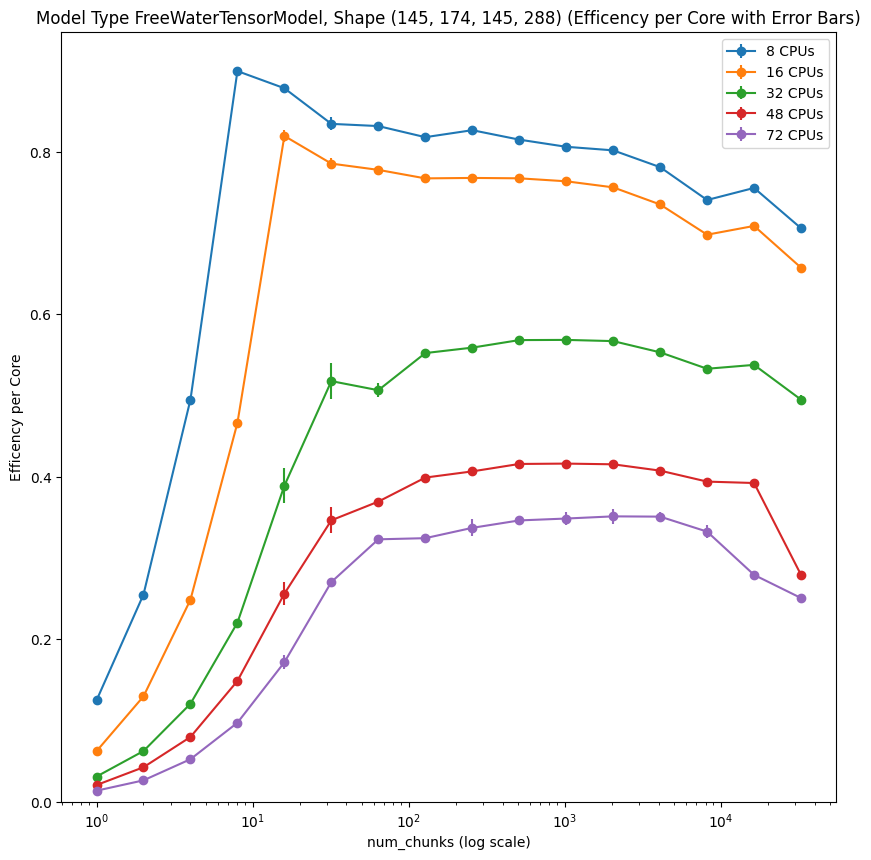
\includegraphics[width=0.8\textwidth,height=0.8\textheight]{figures/fwdtim_efficency.png} \\
\end{longtable}

XXX Plot peak efficiency as a function of number of CPUs for the two
models. The slope is probably related to the cost-per-voxel of each
model (a lot higher for FWDTI).

Ray tends to spill a large amount of data to disk and does not clean up
afterwards. This can quickly become problematic when running multiple
consecuitive models. Withing just an hour or two of running ray could
easily spill over 500gb to disk. We have implemented a fix for this
within our model as follows:

There seems to be an inverse relationship between the computational cost
per voxel and the speedup that you get from parallelization. This is why
CSD speedup is maximal for 32 cores.

XXX We should try to make a theoretical guesstimate of the cost (in \$)
per model with the cost of different machines in mind, making some
assumptions about the differences between a 32-core and a 72-core
machine. We might still come out ahead using 72 CPU machines, given the
cost differential in this kind of calculation..

\begin{Shaded}
\begin{Highlighting}[]
    \ControlFlowTok{if}\NormalTok{ engine }\OperatorTok{==} \StringTok{"ray"}\NormalTok{:}
        \ControlFlowTok{if} \KeywordTok{not}\NormalTok{ has\_ray:}
            \ControlFlowTok{raise}\NormalTok{ ray()}

        \ControlFlowTok{if}\NormalTok{ clean\_spill:}
\NormalTok{            tmp\_dir }\OperatorTok{=}\NormalTok{ tempfile.TemporaryDirectory()}

            \ControlFlowTok{if} \KeywordTok{not}\NormalTok{ ray.is\_initialized():}
\NormalTok{                ray.init(\_system\_config}\OperatorTok{=}\NormalTok{\{}
                    \StringTok{"object\_spilling\_config"}\NormalTok{: json.dumps(}
\NormalTok{                        \{}\StringTok{"type"}\NormalTok{: }\StringTok{"filesystem"}\NormalTok{, }\StringTok{"params"}\NormalTok{: \{}\StringTok{"directory\_path"}\NormalTok{:}
\NormalTok{                         tmp\_dir.name\}\},}
\NormalTok{                    )}
\NormalTok{                \},)}

\NormalTok{        func }\OperatorTok{=}\NormalTok{ ray.remote(func)}
\NormalTok{        results }\OperatorTok{=}\NormalTok{ ray.get([func.remote(ii, }\OperatorTok{*}\NormalTok{func\_args, }\OperatorTok{**}\NormalTok{func\_kwargs)}
                          \ControlFlowTok{for}\NormalTok{ ii }\KeywordTok{in}\NormalTok{ in\_list])}

        \ControlFlowTok{if}\NormalTok{ clean\_spill:}
\NormalTok{            shutil.rmtree(tmp\_dir.name)}
\end{Highlighting}
\end{Shaded}

\section{Discussion}\label{discussion}

\subsection{Acknowledgments}\label{acknowledgments}

This work was funded through NIH grant EB027585 (PI: Eleftherios
Garyfallidis) and a grant from the Chan Zuckerberg Initiative Essential
Open Source Software program (PI: Serge Koudoro).



\end{document}
